%\emph{\emph{•}}
% * <galynazholtkevych1991@gmail.com> 2017-11-19T14:02:18.924Z:
%
% ^.
\documentclass{llncs}
%
\usepackage{amsmath}
\usepackage{amsfonts}
\usepackage{amssymb}
\usepackage{graphicx}
\usepackage{subcaption}
\captionsetup{compatibility=false}
\usepackage{url}
\usepackage[usenames]{color}

\usepackage{lipsum} % stab

\newcommand{\keyterms}[1]{\par{\bfseries{ Key Terms: }}#1}

\begin{document}
\title{Distributed Datastores: Consistency Metric for Distributed Datastores}
\author{Kyrylo Rukkas\and Galyna Zholtkevych}
\institute{V.N.~Karazin Kharkiv National University\\
	4, Svobody Sqr., 61022, Kharkiv, Ukraine\\
	\email{galynazholtkevych1991@gmail.com}}
\maketitle
\begin{abstract}
Distributed databases being evolved require write requests to be handled independently to increase availability.
This means that some number of nodes in a database can process modifying operation. This involves huge conflicts and leads to full inconsistency and mess between replicas. This paper takes attention on the consistency and proposing to replace binary metric by stochastic metric. Also, paper is devoted to 
consistency convergence investigation and propose some inferences for the algorithm of decision-making behaviour.
\end{abstract}

\section{Introduction}\label{sec:intro}
In the epoch of popular usage of IoT, Big Data, Cloud Computing, the data become more and more important thing and require larger, more reliable storage. This leads to increasing size of distributed storages. They become bigger and bigger and require the huge network across all the distributed nodes.
But there are several unsolved problems using large distributed datastores and some of them are strongly related to the CAP-theorem. 
Given that the ACID strategy can not be supported for systems of this class (see \cite{bib:brewer}), mechanisms for delivering data across distributed storage still lack fast eventual consistency convergence, reliability and tolerance to network partitions.

So let's concentrate on efficient consistency model - BASE (Basically Available, Soft State, Eventual Consistency) (see \cite{bib:acid_vs_base}).
Mainly this paper is devoted to eventual consistency. Let us remind what eventual consistency is referencing to well-known book \cite{bib:tanenbaum}: the form of consistency is called eventual if no updates take place for a long time and all replicas will gradually become consistent.

Supporting replicas of an evolving distributed system up-to-date is very important but hard problem. Thus we need to provide a set of indicators of main characteristics of the distributed data store to assess the risk of a wrong decision because of the data inconsistency or unavailability.
In this paper, we focus our study on the problem of estimating data consistency in a distributed data store. Usually, in the datastore consistency is defined as binary for now. We want to demonstrate the useful concept defining of the consistency as binary value. 
For that instead of binary metric for eventual consistency/inconsistency we propose stochastic metric.

Also we would like to know if it is possible to find the optimal interval between writable operations occuring on distributed systems so that system can eventually be consistent in that interval.

In the section \ref{sec:model} we develop consistency model defined in the previous paper \cite{bib:prob_approach} and define the inconsistency metric for a distributed datastore.
In section \ref{sec:complexity} section we approximate the time that is needed for consistency convergence - state of the distributed system when all nodes have consistent replicas.

In section \ref{sec:experiments} we conduct experiments that prove the correctness of metric defined in previous section.
In section \ref{sec:simulation} we provide diagrams of the implemented application that we use for carrying out experiments.

\section{Evolving consistency metric mathematical model: Derived metrics}\label{sec:model}

In the previous paper (see \cite{bib:prob_approach}) we considered the metrics for all three elements of CAP-theorem.
Now our paper is mainly devoted to consistency question and how fast it can converge.
From that paper we are taking the developed mathematical model and expand it with elements, needed for the current research.

We specify it as a tuple $(N, L, \partial,D, r)$, where \\
\begin{tabular*}{\textwidth}{cp{0.5cm}p{0.8\textwidth}}
$N$&& is a finite set of nodes of a distributed datastore; \\
$L$&& is a finite set of links of a distributed datastore; \\
$\partial:L\rightarrow 2^N$&& is a mapping that associates each link with two nodes that it binds;\\
$D$&& is a finite set of stored data units;\\
$r:D\rightarrow 2^N$&& is a mapping that associates each data unit $d$ with a subset of nodes 
that store its replica; \\


$N_d$&& is a finite set of nodes that are having given dataunit $d$; \\
$l(N_d)$&& is a number of nodes in datastore that are having given dataunit; \\
$n_c$&& is a number of nodes in a subset of $N_d$ where all nodes have the same replica.
\end{tabular*}

So we expanded the model now with two last assumptions.

Our mathematical model for inconsistency $I$ will be able to define the inconsistency state of distributed datastore (see Example \ref{ex:metric} and Section \ref{sec:experiments}), and afterwards will focus on time which distributed datastore require to become fully consistent (see Section \ref{sec:complexity}).

For this metric we created the probabilistic event taking two random nodes from the set $N_d$, they can be consistent with some probability. Carrying out this event many times, we can obtain the average probability of that two nodes will be consistent.


Thus, we have the following sample space:

\[\Omega = \{0, 0, 1, 0, 1, 0, 1 , 1, 0, 1, 1, ....\}, \],

where $0$ denotes the event when two nodes are consistent and $1$, on the contrary, when two nodes are inconsistent.

Also let's claim that $p$ is the probability that two nodes are consistent, and
$q = 1 -p$ - the probability that two nodes are inconsistent.


As marked above, we introduce the stochastic metrics for inconsistency/consistency instead of binary ones.
We carry out experiment, we will "freeze" the simulated distributed datastore and time of that "freezing" we call time $t$. Thus we will be able to investigate the current state of the system.

Let's denote  $I$ as a value calculated by probabilistic formula .
We are thinking that having this formula will help us to eventually fully specify the mathematical model for consistency, so let it be one of mathematical model components.
So the probability of that two nodes taken at random are from consistent subset is

\[p_c = \frac{n_c}{l(N_d)} \cdot \frac{n_c - 1}{l(N_d) - 1} = \frac{n_c * (n_c - 1)}{l(N_d)* (l(N_d) -1)},\]
 where $n_c$ is length of consistent subset in the system at time $t$.
Obviously, inconsistency probability then:
\[p_{i} = 1 - p = 1 - \frac{n_c * (n_c - 1)}{l(N_d)* (l(N_d) -1)}.\]
Taking into account that minimum number of consistent nodes will be equal to 1, and the maximum number of consistent nodes is equal to $l(N_d)$, we have following consequences:
\begin{itemize}
\item Two nodes are inconsistent if  $p_{ic} = 1$
\item Two nodes are consistent if $p_{ic} = 0$ 
\end{itemize}

We developed the inconsistency formula for two nodes. Let's now extend it to more general one.
We still suppose that a data unit is represented by replicas on $N_d$ servers. Let's denote it as temporary $N$.
Let we have $K$ classes of mutually consistent replicas.
Then we denote by $N_k$ a number of replicas in $k^\mathrm{th}$ consistency class ($1\leq k<K$).
It is evident that $N_k>0$ for all $k=1,\ldots,K$ and $N=N_1+\ldots+N_K$.
Such representations $N=N_1+\ldots+N_K$ are called integer partitions.


\noindent Thus, in this case any integer partition describes some inconsistency state.

\begin{example}\label{ex:partitions}
All integer partitions for $5$ are
\begin{center}
\begin{tabular}{lclcl}
	5 & & 4+1 & & 3+2\\
	3+1+1 &\hspace*{10pt}& 2+2+1 &\hspace*{10pt}& 2+1+1+1\\
	1+1+1+1+1
\end{tabular}
\end{center}
\end{example}

Taking into account this consideration we define inconsistency metric for a data unit in the term of the corresponding integer partition.
As we denoted above  in the section \ref{sec:model}, we suppose that the studied data unit $d$ is represented by $N$ replicas, which are being described by the integer partition $N=N_1,\ldots,M_K$.

Then the inconsistency metric $I(d)$ is defined by the formula
\begin{equation}\label{eq:metric}
	I(d)=1-\sum_{k=1}^K\dfrac{N_k(N_k-1)}{N(N-1)}.
\end{equation}

\begin{example}\label{ex:metric}
Let us suppose that a data unit $u$ are being stored on five servers.
Then the corresponding inconsistency states (see Example~\ref{ex:partitions}) have the following values of the inconsistency metric
\begin{center}
\begin{tabular}{lclcl}
	$I(5)=0$ & & $I(4+1)=\frac{2}{5}$ & & $I(3+2)=\frac{3}{5}$\\
	$I(3+1+1)=\frac{7}{10}$ &\hspace*{10pt}& $I(2+2+1)=\frac{4}{5}$
		&\hspace*{10pt}& $I(2+1+1+1)=\frac{9}{10}$\\
	$I(1+1+1+1+1)=1$
\end{tabular}
\end{center}
The meaning of $I(d)$ is the value of probability to establish the fact of inconsistency by the way of comparison two randomly chosen replicas.
\end{example}
Example~\ref{ex:metric} demonstrates that the proposed metric is equal to $0$ for the absolutely consistent data unit (the case 5) and is equal to $1$ for the absolutely inconsistent data unit (the case 1+1+1+1+1) in the subset $N_d$.


\section{Convergence time complexity}\label{sec:complexity}

Now we are interested to calculate the time that can be taken for consistency convergence.
We want to prove the following:
\begin{proposition}\label{prop}
Let we have a distributed datastore where all links are available and reliable (network partitions do not happen in a datastore and nodes are stable and respond in approximately equal time); the interval between writing operations is $t_w$.
Then $t_w$ is less than the diameter of network graph ensures eventual consistency of the datastore.
\end{proposition}
\begin{proof}
Let us denote as $T_c$ time for consistency convergence (time that is needed for the whole system to become consistent).
Let we have the trivial network where all links have capacity 1.
Thus, as the input we have the connected graph
$G$ with set of nodes $N$ and set of edges $E$. 
\par\noindent Let us assume now that weight of each edge $e\in E$ satisfies the equality $w(e) = 1$\,.
\par\noindent
Let us take the nodes $n_1$ and  $n_2$ that are at the largest distance each from other. So we can count that the time of delivering replica between $n_1$ and $n_2$ is the shortest path from $n_1$ to $n_2$.
Extrapolating this to all the system and taking into account that in the distributed datastore nodes are broadcasting each to other in parallel,  we obtain the upper boundary of $T_c$ is the maximum of shortest paths in the worst case.
It is well-known that such maximum is diameter of the graph $T_c = diameter(G)$.
\par\noindent Let us complicate the system introducing the different capacity for links in distributed datastore that means that now our graph $G$ is weighted and 
$w(e) \in\mathbb{N}$ for all $e\in E$.
\par\noindent
Thus, the diameter is the path $P = [e_1....e_n]$ where $e_i$ has own weight and
\[
	T_c = \sum_{i=1}^{n}w_i
\]
where $w_i$ is the weight of edge $e_i$ of the path $P$.
\par\noindent
$T_c$ is the number of time slots that a datastore requires to become fully consistent.
This means that after $T_c$ time points, all replicas become consistent.
This also means that a datastore is again available to accept writing requests, so that datastore will be able to store all the replicas passed before, and no accidental updating happen in the meantime.
\qed
\end{proof}

\section{Case Study}\label{sec:experiments}

The study in the Section \ref{sec:model} had been checked by the following experimentation: 
we implemented a code that allows to test the accuracy of the inconsistency metric. Probability intervals for different partitions are demonstrating that the formula is correct - values obtained are around values obtained theoretically. To be more intuitive we took the same number of nodes and same partitions.

It is obviously that we do not have exact matching, because the experiment is based on number of iterations where two nodes are taken from a given set of nodes randomly, but all we need is that value should vary slightly around theoretical value. Look in the figures below:
%
\begin{figure}[p]
\begin{subfigure}{0.5\linewidth}
\centering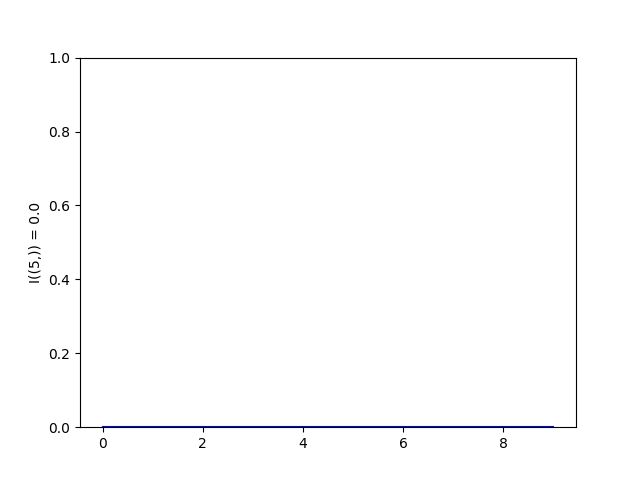
\includegraphics[scale=0.4]{images/1-consistent-partition.png}\hfill
\end{subfigure}
\begin{subfigure}{0.5\linewidth}
\centering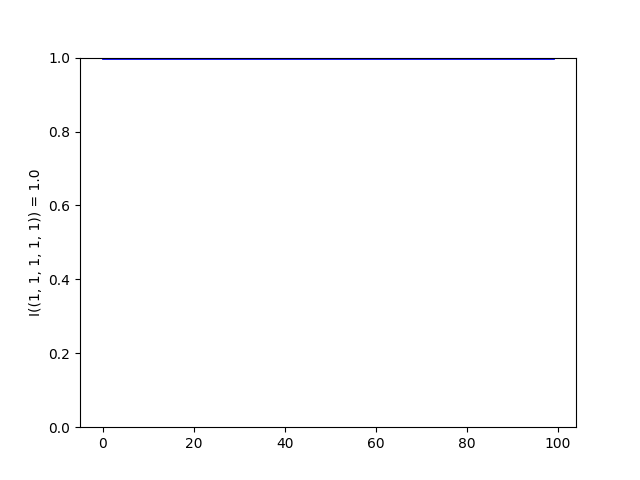
\includegraphics[scale=0.4]{images/1-1-1-1-1-consistent-partitions-probability.png}
\end{subfigure}
\caption{The datastore is fully consistent and fully inconsistent}\label{pic:fully}
\end{figure}
%
Firstly, it can be seen that for one consistent partition $I(d)$ is equal to $0$ and when the system is fully inconsistent $I(d)$ is equal to $1$ (see in Fig~\ref{pic:fully}).

\begin{figure}
\begin{subfigure}{0.5\linewidth}
\centering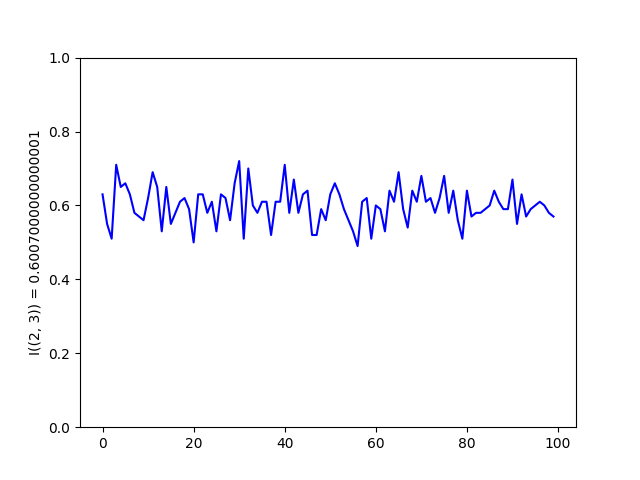
\includegraphics[scale=0.4]{images/2-3-consistent-partitions-probability.png}\hfill
\end{subfigure}
\begin{subfigure}{0.5\linewidth}
\centering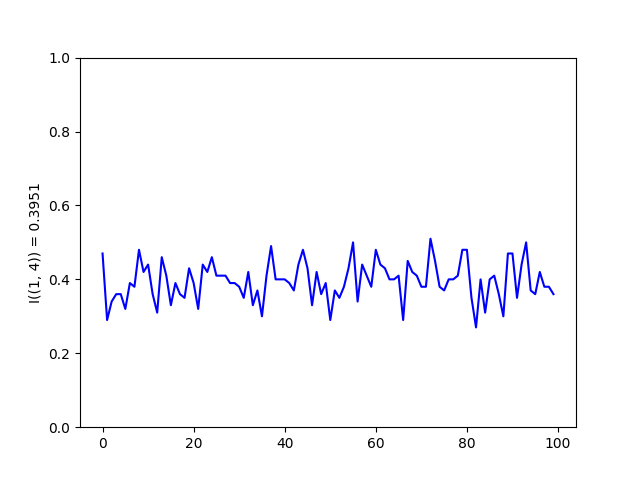
\includegraphics[scale=0.4]{images/1-4-consistent-partitions-probability.png}
\end{subfigure}
\caption{The datastore has two consistent partitions}\label{pic:two_parts}
\end{figure}
Let us compare now the situation when we have two consistent partitions: the set which contains 2 and 3 nodes that consistent in the own subset, and the set with 4 and 1-length consistent subsets (see results in Fig~\ref{pic:two_parts}).

Then we can easily see that:
\[
	I(3,2) = 1 - \frac{3 \cdot 2}{5 \cdot 4} - \frac{2 \cdot 1}{5 \cdot 4} = \frac{3}{5} ,
\]
and
\[
	I(4,1) = 1 - \frac{4 \cdot 3}{5 \cdot 4} - \frac{1 \cdot 0}{5 \cdot 4} = \frac{2}{5} ,
\]
Following this procedure for three consistent partitions (presented in 
Fig~\ref{pic:three_parts}) in $N_d$:
\[
	I(3,1,1) = 1 - \frac{3 \cdot 2}{5 \cdot 4} - \frac{1 \cdot 0}{5 \cdot 4} - \frac{1 \cdot 0}{5 \cdot 4} = \frac{7}{10} ,
\]
and 
\[
	I(2,2,1) = 1 - \frac{2 \cdot 1}{5 \cdot 4} - \frac{2 \cdot 1}{5  \cdot 4} - \frac{1 \cdot 0}{5 \cdot 4} = \frac{4}{5} .
\]

\begin{figure}[p]
\begin{subfigure}{0.5\linewidth}
\centering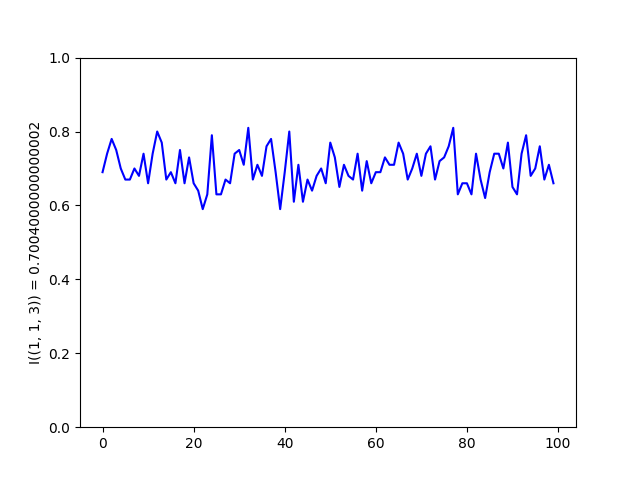
\includegraphics[scale=0.4]{images/1-1-3-consistent-partitions-probability.png}
\end{subfigure}
\begin{subfigure}{0.5\linewidth}
\centering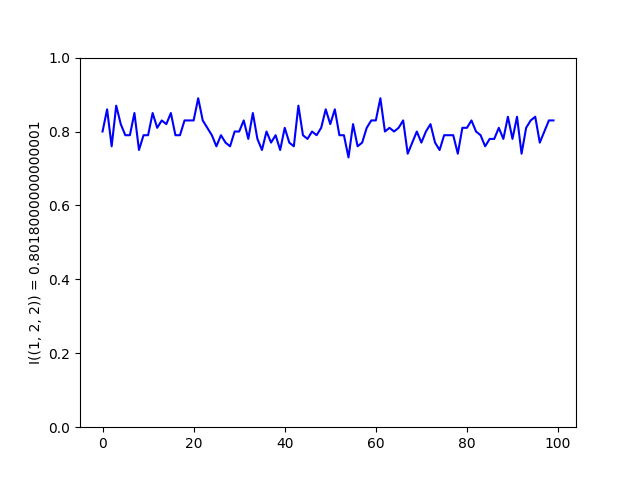
\includegraphics[scale=0.4]{images/1-2-2-consistent-partitions-probability.png}
\end{subfigure}
\caption{The datastore has three consistent partitions}\label{pic:three_parts}
\end{figure}
%
And the final one:
\[
	I(2,1,1,1) = 1 - \frac{2 \cdot 1}{5 \cdot 4} - 3\cdot\frac{1 \cdot 0}{5 \cdot 4} = \frac{9}{10}\,.
\]
See results in Fig~\ref{pic:four_parts}.
\begin{figure}
\centering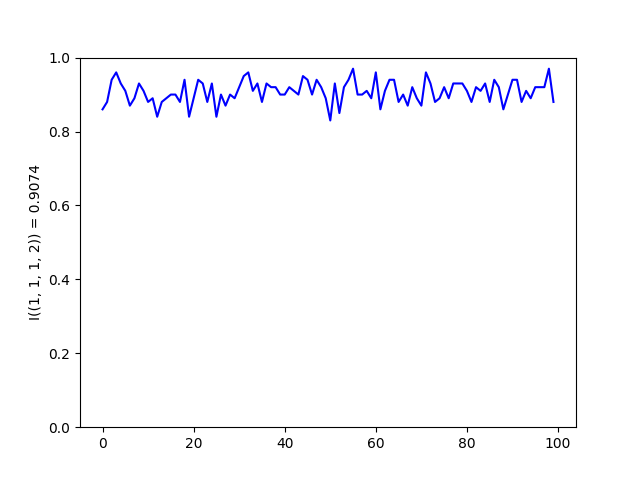
\includegraphics[scale=0.4]{images/1-1-1-2-consistent-partitions-probability.png}
\caption{The datastore has four consistent partitions}\label{pic:four_parts}
\end{figure}
%
So, we had easily shown on a simple subset, that our inconsistency metric value corresponds to theoretical one.

Now we present the graphic that demonstrates the verity of that claim we did in Section \ref{sec:complexity} about that consistency convergence time $T_c$ for graph $G$ will be no greater than diameter of $G$.
To be more intuitive, we carried out the set of experiments on our simulation model: having simulated distributed datastore, we easily could run the imitation of one message broadcasting through the datastore and calculate the number of time slots it is taking in the real time. We have done it for graph with each edge of capacity 1. Below there are graphics for 100, 200, 1000 experiments (see in Fig~\ref{pic:100}, \ref{pic:200}, \ref{pic:1000}).

We draw graphics in the following manner: obtain the diameter of graph $G$ (ordinates) and calculated by the simulation $T_c$ (axis). We can easily see that either we have the line demonstrating that $T_c = D(G)$, or
points that are showing that $T_c < D(G)$.
%
\begin{figure}[p]\label{pic:diagram}
\begin{subfigure}{0.3\linewidth}
\centering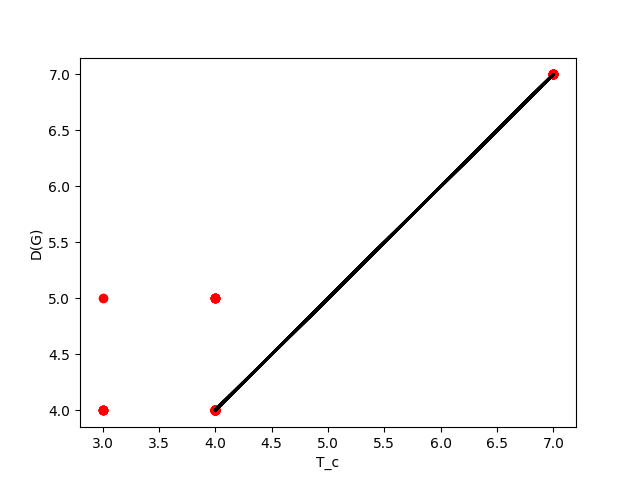
\includegraphics[width=\linewidth]{images/100-consistency-convergence.png}
\caption{100 experiments}\label{100}
\end{subfigure}
\begin{subfigure}{0.3\linewidth}
\centering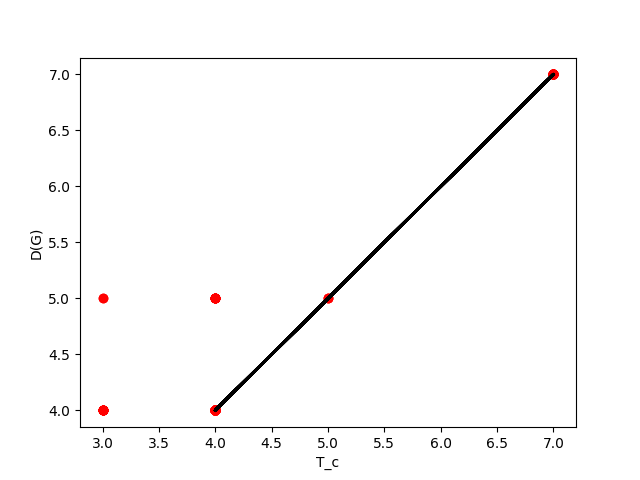
\includegraphics[width=\linewidth]{images/200-consistency-convergence.png}
\caption{200 experiments}\label{200}
\end{subfigure}
\begin{subfigure}{0.3\linewidth}
\centering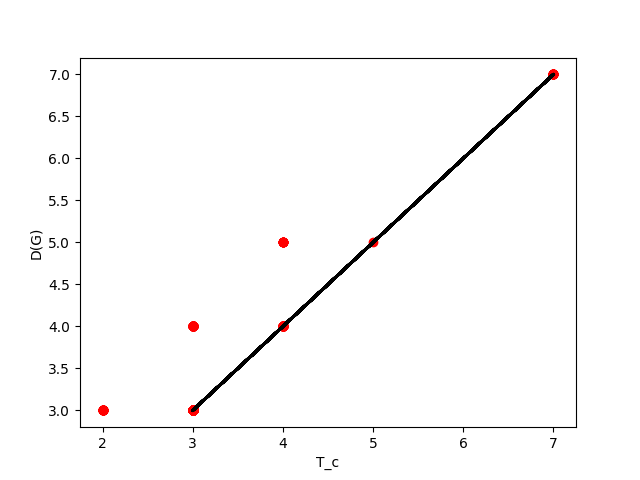
\includegraphics[width=\linewidth]{images/1000-consistency-convergence.png}
\caption{1000 experiments}\label{1000}
\end{subfigure}
\caption{Graphics for consistency convergence time}
\end{figure}
%
In this section we consider the case of an unweighted graph. 
But the general situation requires to consider weighted one.
In this case, weight of an edge means the average time for delivering a message via the corresponding link.
However, algorithms to simulate this case are more complex.
Therefore this general case will be considered in the future, expanding experiments for random regular graph. Now we are able to present some results for random regular graph, that substantiate our Prop~\ref{prop} in the general case (
see in Fig~\ref{pic:100-w}, \ref{pic:200-w}, \ref{pic:1000-w}).

We can observe that all points have a location in the graphics such that $T_c$ is less or equal to $D(G)$  for weighted random regular graph.
\begin{figure}[p]\label{pic:diagram}]
\begin{subfigure}{0.3\linewidth}
\centering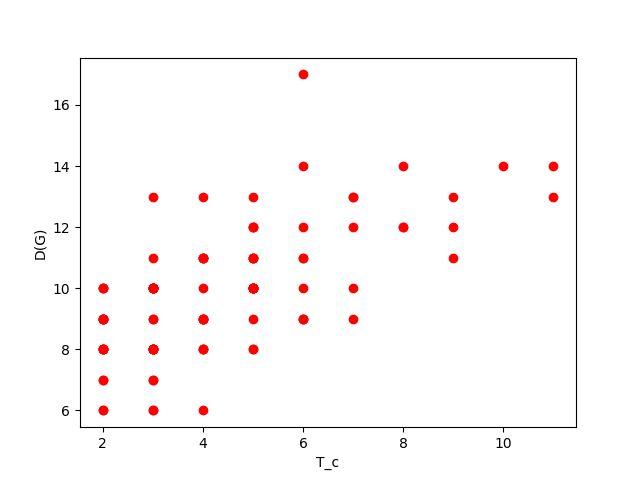
\includegraphics[width=\linewidth]{images/100-consistency-convergence-weighted.png}
\caption{100 experiments}\label{pic:100-w}
\end{subfigure}
\begin{subfigure}{0.3\linewidth}
\centering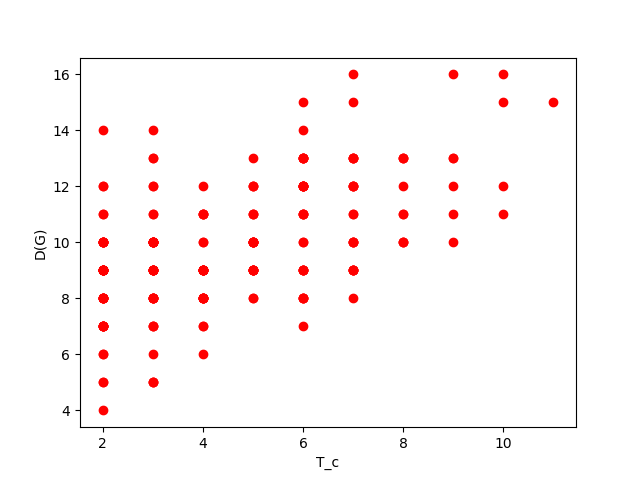
\includegraphics[width=\linewidth]{images/200-consistency-convergence-weighted.png}
\caption{200 experiments}\label{pic:200-w}
\end{subfigure}
\begin{subfigure}{0.3\linewidth}
\centering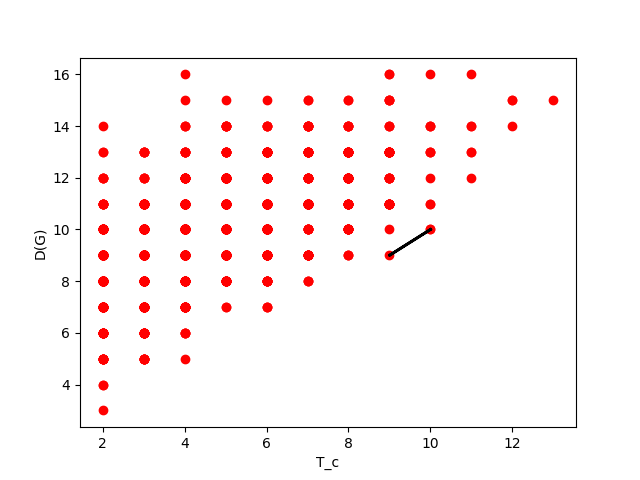
\includegraphics[width=\linewidth]{images/1000-consistency-convergence-weighted.png}
\caption{1000 experiments}\label{pic:1000-w}
\end{subfigure}
\caption{Graphics for consistency convergence time on weighted graph}
\end{figure}
%
\section{Simulation Model to Estimate Inconsistency Ratio of Data}\label{sec:simulation}
To carry out our experiments, we needed to implement the simulation model that will do experiment and calculate all needed values. This model is implemented as a computer program in Python language. We are thining that it is not valuable to present all the code of the program (however it is available at github page \cite{bib:github_dds}), but we count that it is useful to present the short class diagram of the project (see Fig~\ref{pic:diagram} below).
\begin{figure}
\centering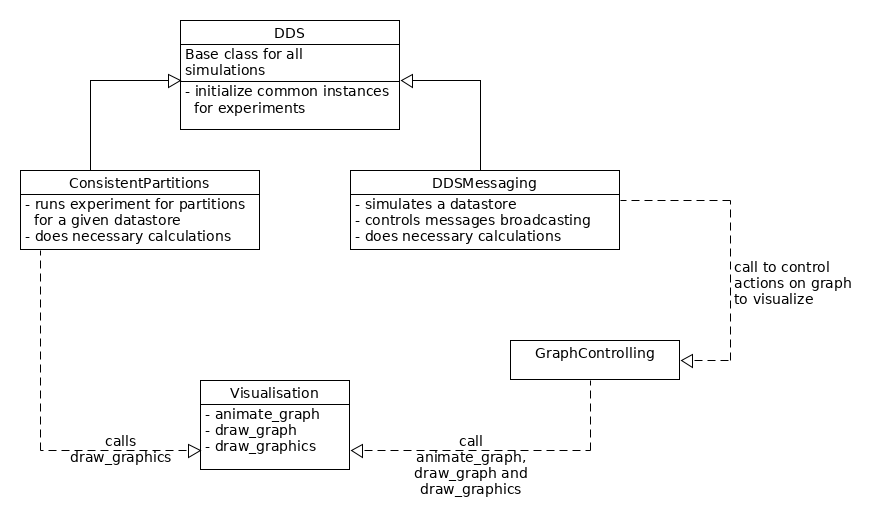
\includegraphics[scale=0.4]{images/dds-class-diagram.png}
\caption{Class diagram for simulation model of a distributed datastore}
\label{pic:diagram}
\end{figure}
%
Also we would like to present the state machine diagram for the algorithm that was implemented to carry out experiments of consistency convergence estimation on a distributed datastore (see Fig~\ref{pic:state-machine}).
\begin{figure}[t]
\centering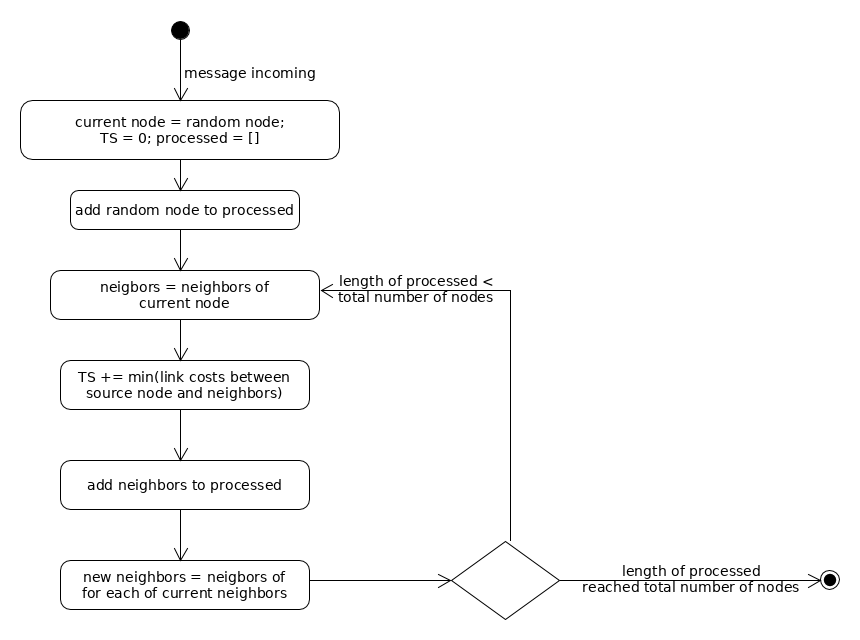
\includegraphics[scale=0.4]{images/message-broadcasting-state-machine.png}
\caption{State machine of simulation of message broadcasting through a datastore}\label{pic:state-machine}
\end{figure}
%
For experiment simulation we had chosen random regular graph.
During simulation we could see that for degree great than 2, calculating the time-slots taken for consistency convergence for one iteration, we can take a minimum between paths to neighbors and it will be the correct choice. Because for regular graph if the path to another neighbor is greater, there will be another path with lesser link cost that will take less time to converge.
%
\section{Conclusion}
In this paper we have studied the consistency property for distributed datastores.
So thinking how huge distributed datastores could be and having small interval between write operations to a datastore, we can conclude that binary variable loses its utility.
It might be needed to evaluate current inconsistency state of a datastore, to get nodes that are consistent and make a decision based on obtained results.

Therefore we have proposed stochastic metric instead of binary one considering consistent partitions of a distributed datastore, formed metric for the inconsistency and shown the correctness of the formulae by carrying out experiments, shown when distributed datastore is fully inconsistent and fully consistent, evaluated the upper boundary of time that is taken for consistency convergence in a distributed datastore, taking into account that datastore is reliable, stable and does not have network partitions.

Thus, based on the research of current paper we can make following recommendations for those who build the network topology of the distributed datastore:
\begin{itemize}
\item in the case of your datastore is a system with a domination of read operations, it must be sufficient to choose such network topology where frequency of write operations will be no greater than diameter of the graph representing network topology of a distributed datastore;
\item if frequency of write operations is grater than diameter of the graph, it may be useful to evaluate current inconsistency state of the graph;
\item if inconsistency state is close to 0 enough for current requirements, it means that there are inconsistent nodes that are far enough to not conflict with new replicas. Thus, developer or administrator of a datastore  can choose as source availiable for writing that node that is in consistent list and far enough for inconsistent ones. But for that developer needs to provide such an algorithm for a datastore so that he will be able to obtain the current list of consistent nodes;
\item if still more strict consistency needs to be satisfied and inconsitency state is close enough to 0, a developer or administrator of a datastore can choose as source node for writing the node closest to the source node where previous write operation occurred;
\item if replica's history is not important for requirements, it may be possible to solve the problem fixing conflicts. This problem has been investigated in this paper \cite{bib:c_ts}
\end{itemize}
Above we described that we considered a lot of useful things for consistency in a distributed datastore. But still the research in this direction need to be continued and we have formed the next goals for the the future research
\begin{itemize}
\item carry out experiments for inconsistency metric in the worst case;
\item complicate a datastore introducing different availability for each node;
\item complicate a datastore introducing various network partitions for a datastore;
\item provide an algorithm that will allow to make a decision what is the best approach for a given datastore such that the eventually consistency is satisfied or an approach when inconsistency will not impact on datastore requirements;
\item theory for finding the most actual replica and time complexity for this algorithm
\item consider all the proposed above metrics in various kinds of real topologies.
\end{itemize}

\begin{thebibliography}{00}
\bibitem{bib:brewer}
Eric A. Brewer:
Towards robust distributed systems,
(Invited talk). Principles of Distributed Computing, Portland, Oregon (July 2000).

\bibitem{bib:prob_approach}
Kyrylo Rukkas, Galyna Zholtkevych:
Distributed Datastores: Towards Probabilistic Approach for Estimation of Dependability,
ICTERI 2015: 523-534

\bibitem{bib:acid_vs_base}
Charles Roe:
ACID vs. BASE: The Shifting pH of Database Transaction Processing
http://www.dataversity.net/acid-vs-base-the-shifting-ph-of-database-transaction-processing, March 1, 2012

\bibitem{bib:tanenbaum}
Tanenbaum, A.S., Van Steen, M.:
Distributed systems. Principles and Paradigms (2nd Edition).
Prentice-Hall, Inc. (2006)

\bibitem{bib:andrews}
Andrews,~G.\,E.:
The theory of partitions.
Addison-Wesley (1976)


\bibitem{bib:github_dds}
G.Zholtkevych: 
DDS Simulation project,
https://github.com/gzholtkevych/DDS-Simulation (2016) 

\bibitem{bib:c_ts}
Sanjay Kumar Madria: 
Handling of Mutual Conflicts in Distributed Databases using Timestamps,
The Computer Journal. Vol. 41, No.\,6 (1998) 

\end{thebibliography}
\end{document}

